\documentclass[11pt]{article}
\usepackage[margin=1in]{geometry}
\usepackage{listings}
\usepackage{graphicx}
\usepackage{subfigure}
\usepackage{subcaption} % For subfigures
\usepackage{float} % for H option in figures
\usepackage{hyperref}
\usepackage[htt]{hyphenat} % for non-overflowing texttt

\usepackage{listings}

\title{Description of Source Data}
\author{Anton Zhitomirsky}

\usepackage{biblatex} %Imports biblatex package
\addbibresource{../../../source/bibliography.bib} %Import the bibliography file

\begin{document}

\maketitle

\section{Structure of source Data}

Results are structured in the file:

\begin{lstlisting}[language=bash]
/vol/biomedic3/bglocker/nnUNet
\end{lstlisting}

\begin{lstlisting}[language=inform]
-rwxr-xr-x   1 bglocker biomedia 236 Sep 24 15:16 exports
drwxr-sr-x   9 bglocker biomedia   9 Nov 25 10:55 nnUNet_preprocessed
drwxr-sr-x   9 bglocker biomedia  10 Nov 25 10:50 nnUNet_raw
drwxr-sr-x   9 bglocker biomedia   9 Nov 25 12:20 nnUNet_results
drwxr-sr-x  11 bglocker biomedia  11 Dec 16 09:10 nnUNet_testing
-rw-r--r--   1 bglocker biomedia 644 Oct 20 07:20 run_nnunet_0.sh
-rw-r--r--   1 bglocker biomedia 644 Oct 20 07:20 run_nnunet_1.sh
-rw-r--r--   1 bglocker biomedia 644 Oct 20 07:20 run_nnunet_2.sh
-rw-r--r--   1 bglocker biomedia 644 Oct 20 07:21 run_nnunet_3.sh
-rw-r--r--   1 bglocker biomedia 644 Oct 20 07:21 run_nnunet_4.sh
\end{lstlisting}

\section{nnUNet\_raw}\label{section:raw}

nnUNet\_raw has the original (training) images with manual annotations. Each Dataset below is treated as a binary segmentation problem. See Section\ref{section:itksnap}

\begin{lstlisting}[language=inform]
drwxr-sr-x  4 bglocker biomedia   5 Sep 17 13:47 Dataset001_Anorectum
drwxr-sr-x  3 bglocker biomedia   5 Sep 17 20:24 Dataset002_Bladder
drwxr-sr-x  3 bglocker biomedia   5 Sep 17 20:27 Dataset003_CTVn
drwxr-sr-x  3 bglocker biomedia   5 Sep 17 20:28 Dataset004_CTVp
drwxr-sr-x  3 bglocker biomedia   5 Sep 17 20:29 Dataset005_Parametrium
-rw-r--r--  1 bglocker biomedia 135 Nov 25 10:50 note
\end{lstlisting}

\section{nnUNet\_results}

The raw files from Section\ref{section:raw} are used to train an \href{https://github.com/MIC-DKFZ/nnUNet}{nnUNet model}. Which does a 5-fold cross validation, resulting in five models, each trained on 80 subjects and tested on 20 (there is a total of 100 subjects with manual annotations).

\subsection{Script}

\subsubsection*{Slurm script}

Each of the scripts are presented as bash scripts in \texttt{/vol/biomedic3/bglocker/nnUNet/run\_nnunet\_*.sh}. These are used to schedule the python program into the Slurm scheduler for running in the cloud.

\begin{lstlisting}[language=bash]
#!/bin/bash

# Example of running python script in a batch mode
#SBATCH -c 4                        # Number of CPU Cores
#SBATCH -p gpus                     # Partition (queue)
#SBATCH --gres gpu:1                # gpu:n, where n = number of GPUs
#SBATCH --mem 12288                 # memory pool for all cores
#SBATCH --nodelist lory          	# SLURM node
#SBATCH --output=slurm.%N.%j.log    # Standard output and error log

# Source virtual environment (pip)
source /vol/biomedic3/bglocker/coding/envs/nnunet/bin/activate

# Set env variables
source /vol/biomedic3/bglocker/nnUNet/exports

# Run python script
nnUNetv2_train 1 3d_fullres 4 # where 4 refers to which dataset we're 
                              # training
\end{lstlisting}

\begin{itemize}
    \item Source virtual environment
    
    This is activating the already created python environment. 

    \item Set env variables
    
    contains paths for raw, results and preprocessed directories

    \item Run python scripts 
    
    runs the script at \texttt{/vol/biomedic3/bglocker/coding/envs/nnunet}
\end{itemize}

\subsubsection*{Python script}

No access

\section{nnUNet\_testing}

The models are then tested against 10 hold out manual semgentations with no manual segmentations.

\section{Viewing the Data}\label{section:itksnap}

The viewing tool used is ItkSnap, which was developed as an open source tool for viewing medical imaging scans. The view (Figure\ref{fig:view}) shows how you would see input data.

\begin{figure}[H]
    \centering
    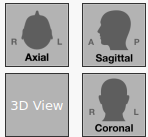
\includegraphics[]{images/view.png}
    \caption{view of all input data}\label{fig:view}
\end{figure}

With that we can use this tool to view input data. Here, the R and L stand for right and left respectively, and the A and P stand for Anterior and Posterior. We can provide a few other examples of viewing data displayed below in Figure\ref{fig:AnorectumImage}. We are further provided with manual annotation of the substructures. Figure\ref{fig:AnorectumLabel} shows an example of the annotation of the Anorectum. You can enable the 3D visual model through \texttt{Edit > 3D Panel > Toggle 3D view}.

\begin{figure}[H]
    \centering
    \captionsetup{width=0.45\textwidth}
    \begin{minipage}{.5\textwidth}
        \centering
        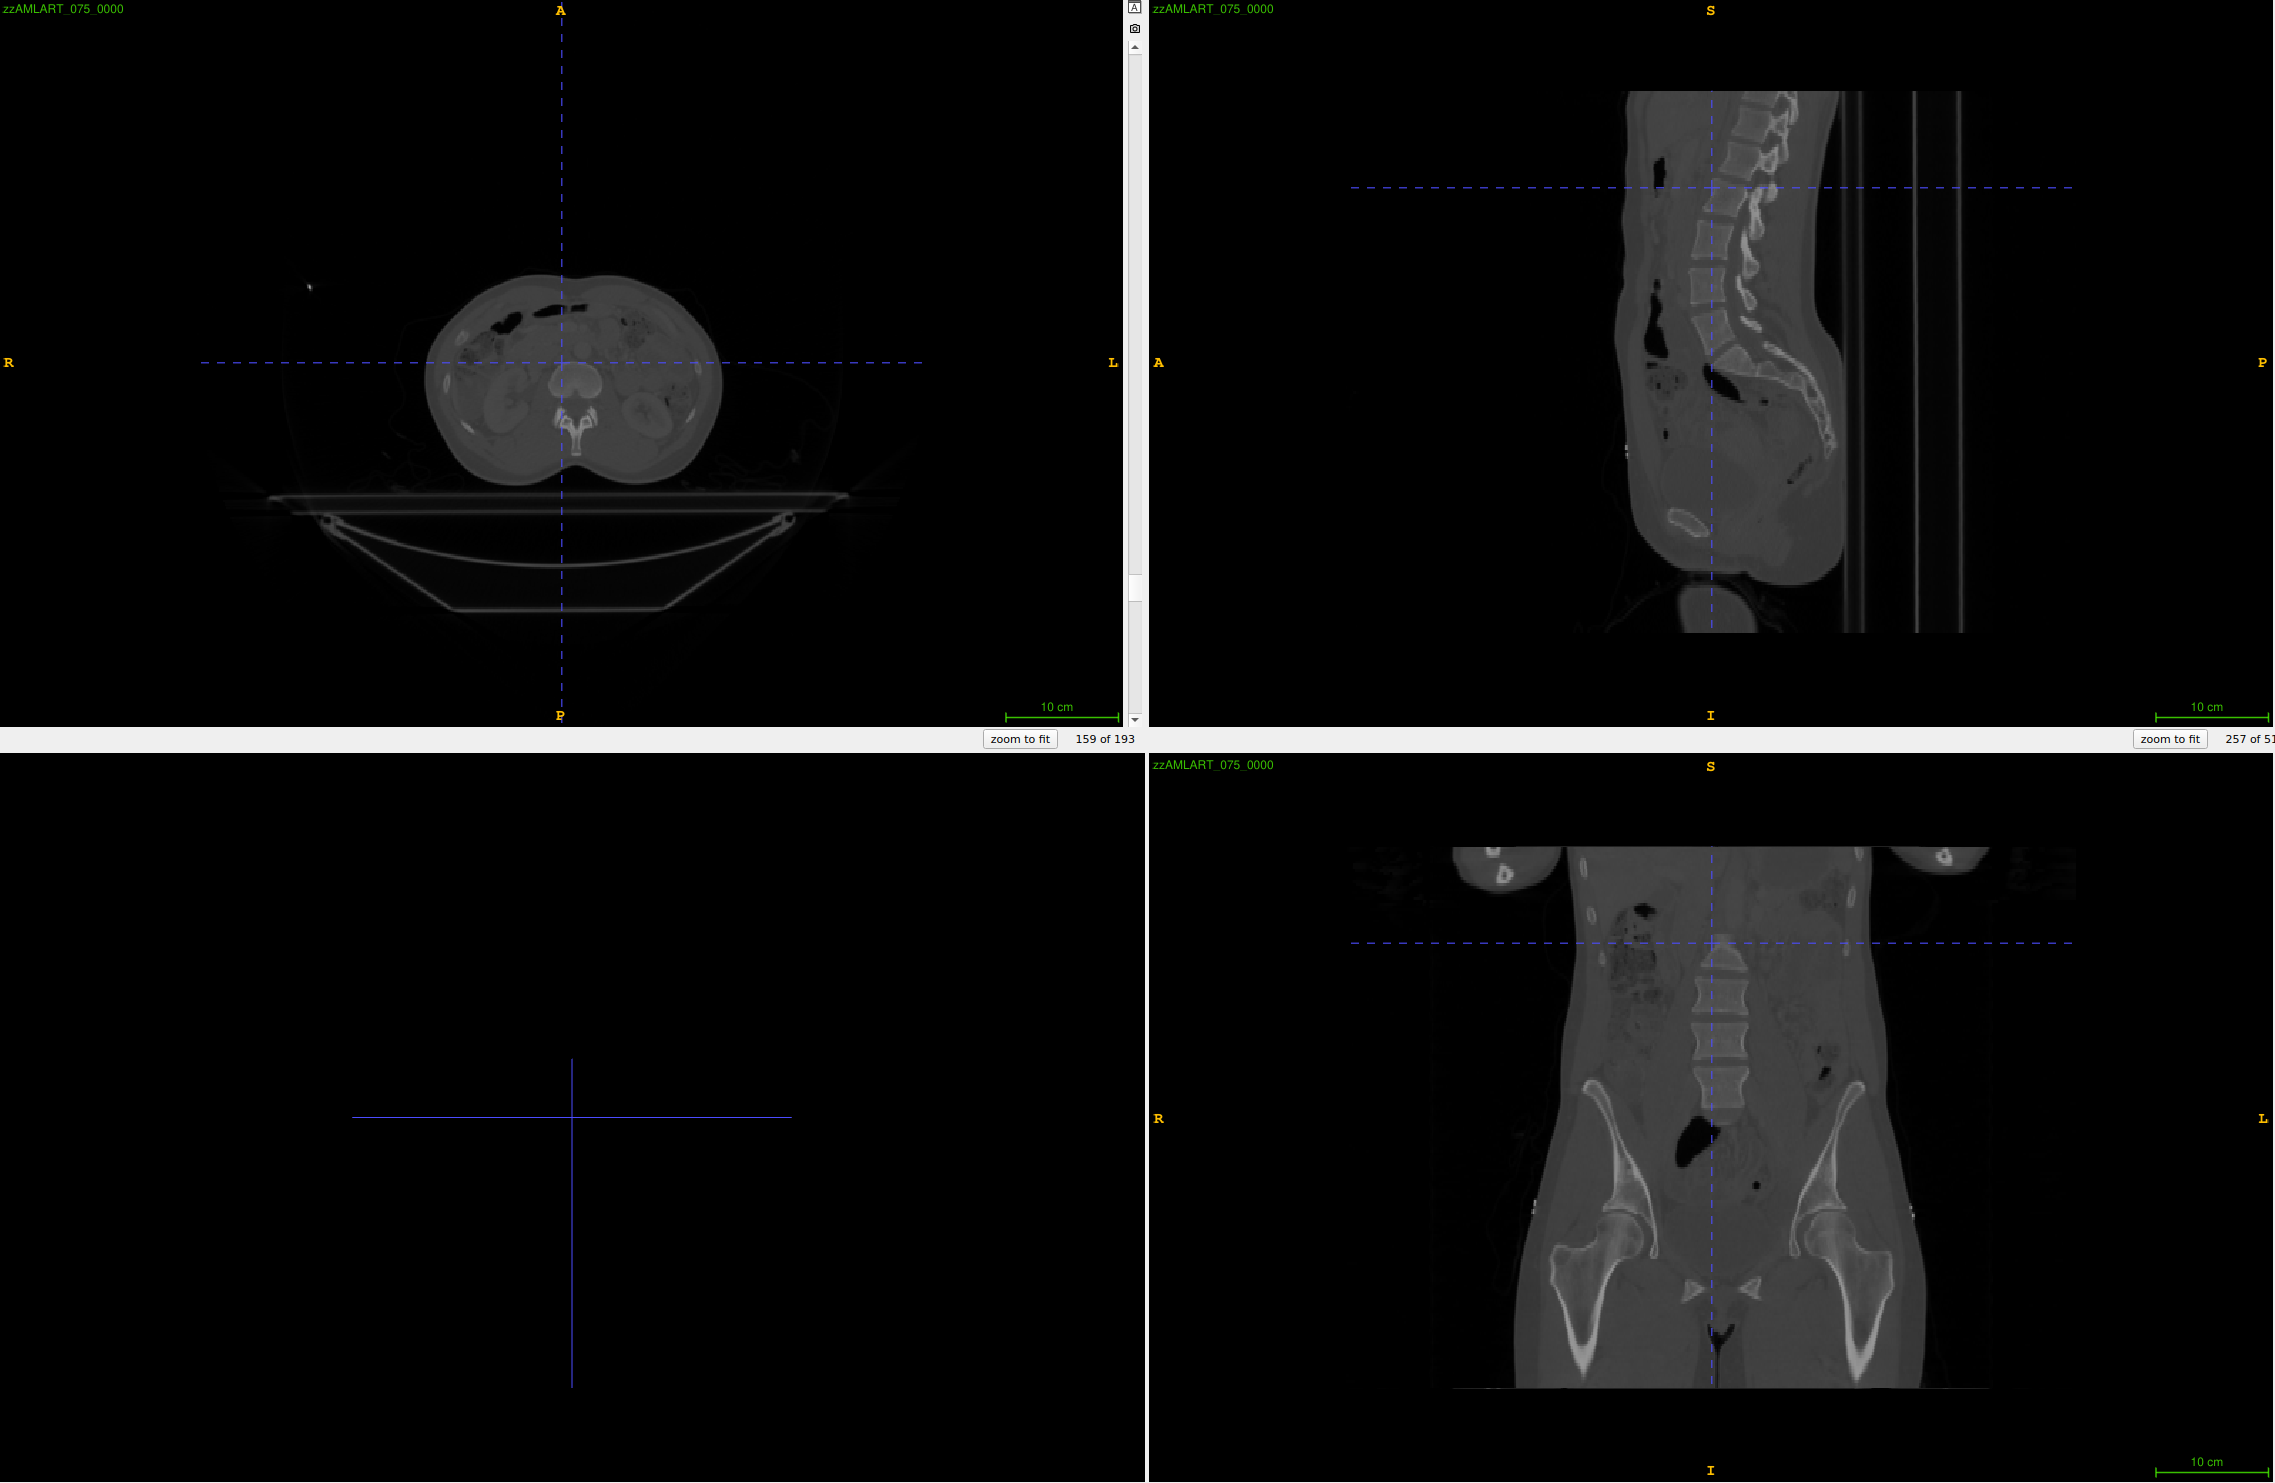
\includegraphics[width=\linewidth]{images/AnorectumImage.png}
        \caption{ItkSnap view of the Anorectum Raw Image}\label{fig:AnorectumImage}
    \end{minipage}%
    \begin{minipage}{.5\textwidth}
        \centering
        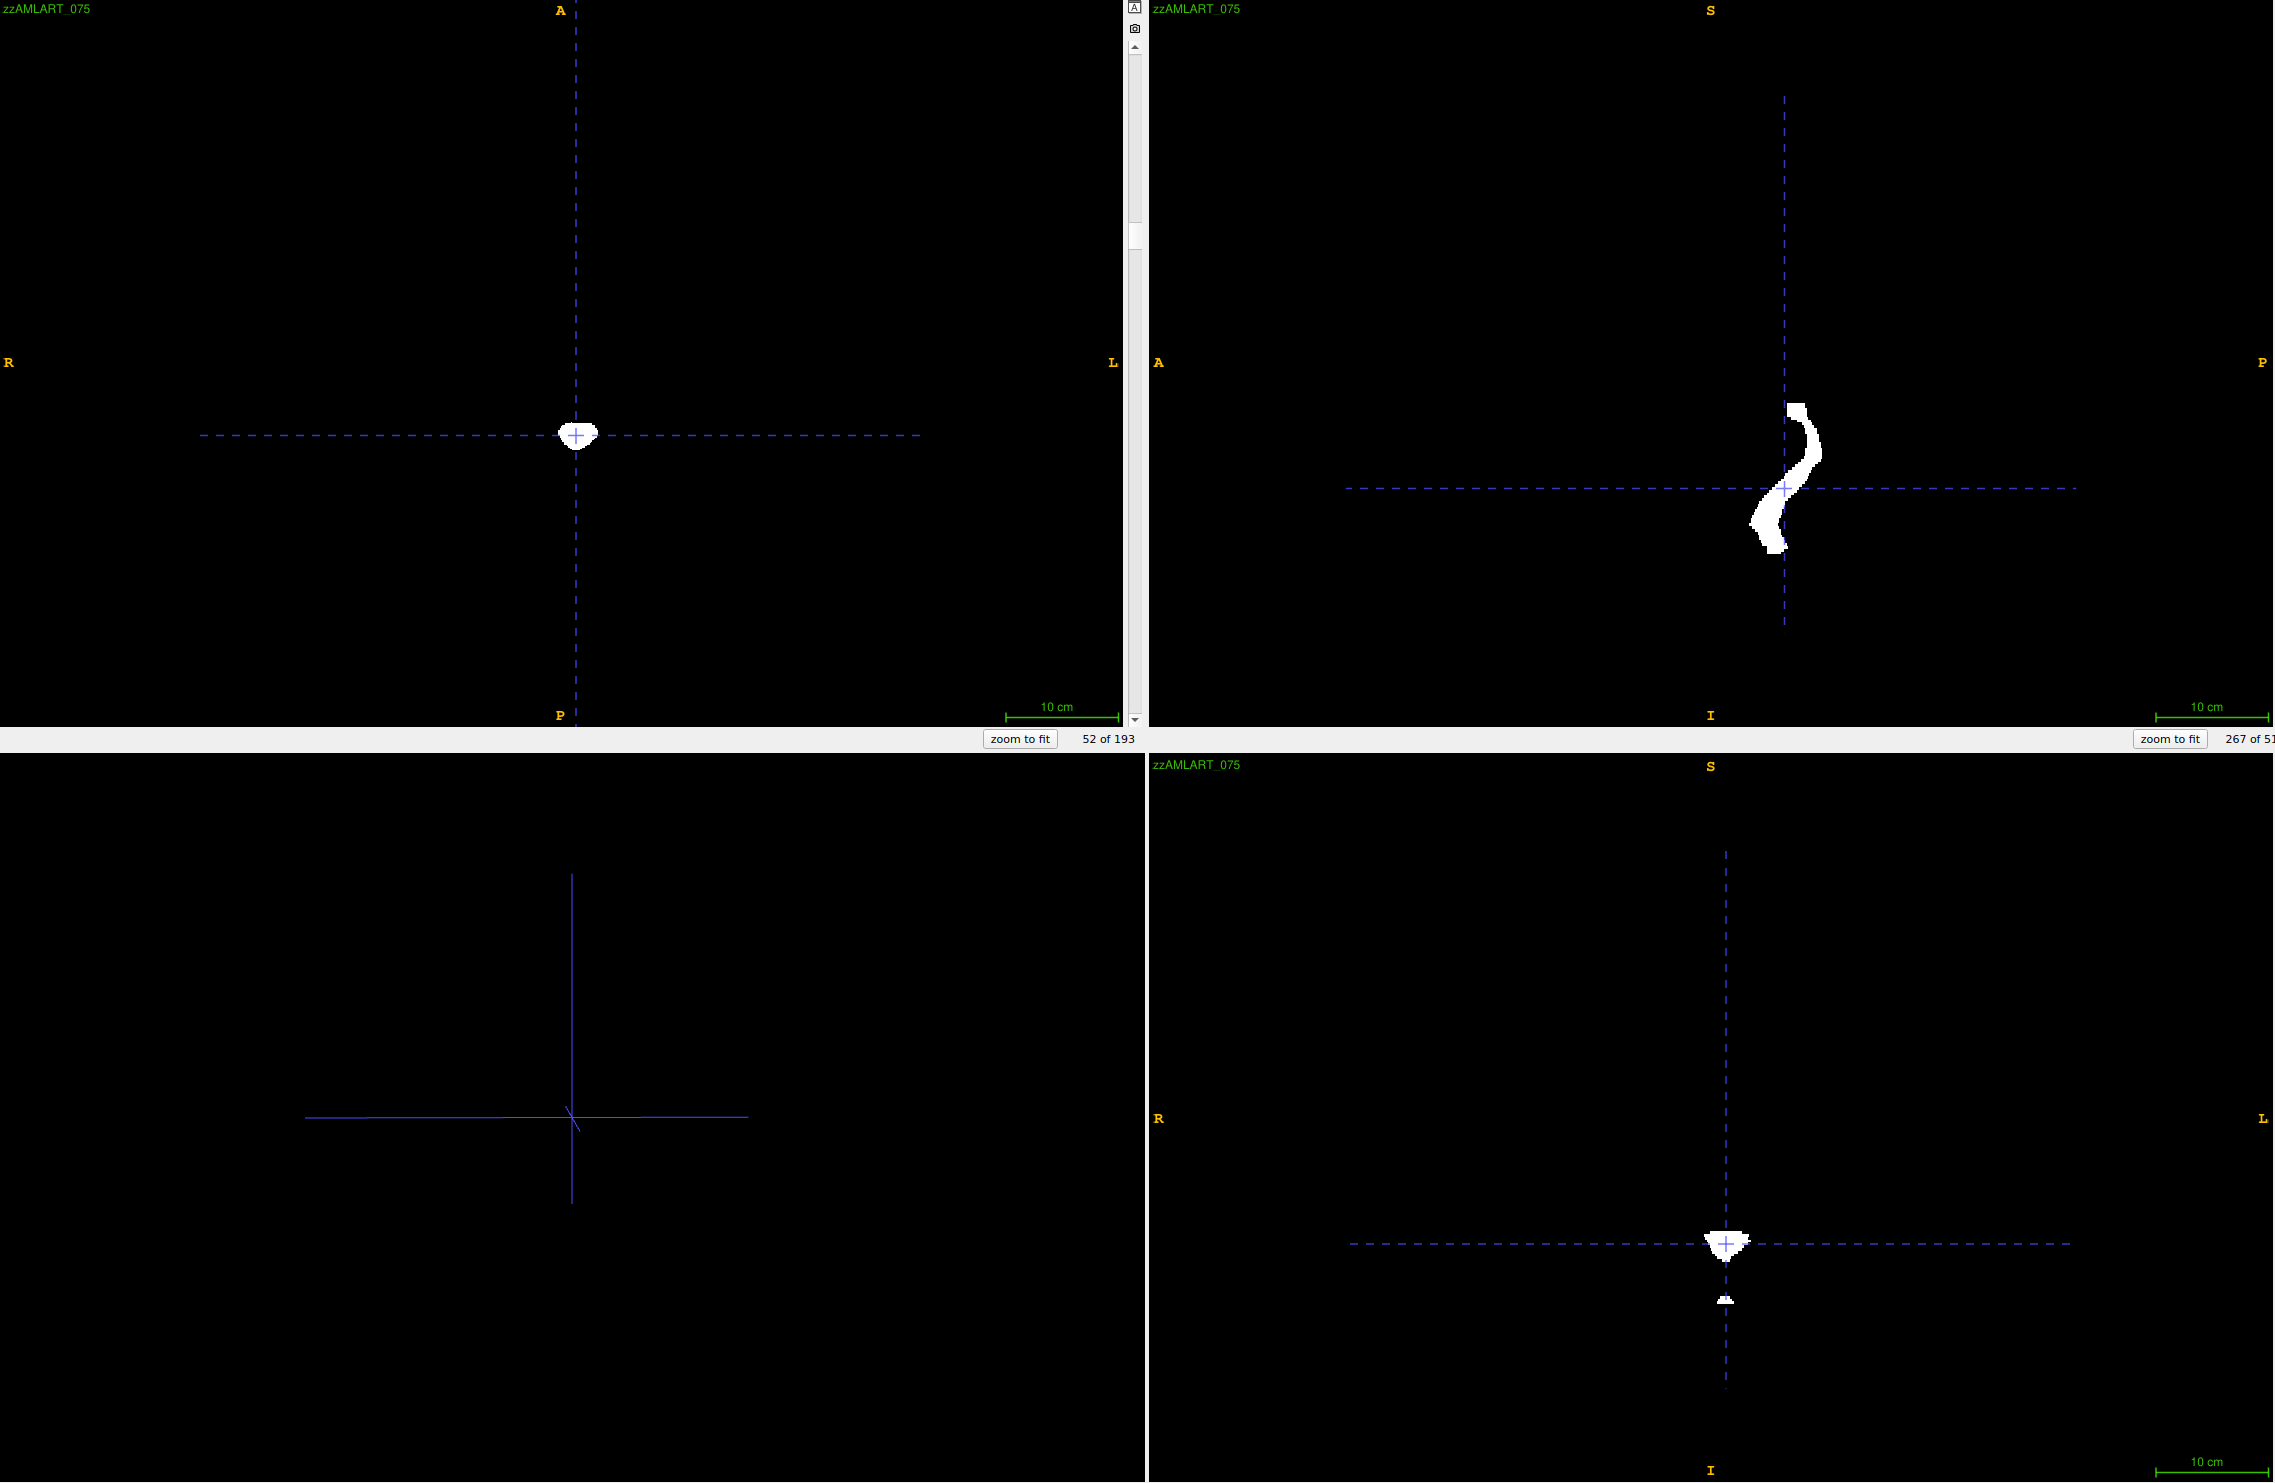
\includegraphics[width=\linewidth]{images/AnorectumLabel.png}
        \caption{ItkSnap view of the Anorectum Raw Image}\label{fig:AnorectumLabel}
    \end{minipage}%
\end{figure} 

\end{document}